\documentclass{beamer}

% Thème
\usecolortheme{whale}

% Packages
\usepackage{lmodern}
\usepackage{amsfonts, amsmath, amssymb, mathrsfs}
\usepackage{enumitem}
\usepackage{graphicx}
\usepackage{pdfpages}
\usepackage{caption, subcaption}

% Barre Pied de page
\setbeamertemplate{footline}{
  \begin{beamercolorbox}[wd=\paperwidth,ht=2.25ex,dp=1ex]{author in head/foot}
    \usebeamerfont{author in head/foot}
    \hspace*{2ex}\insertauthor \hfill \inserttitle \hfill \insertdate \hfill \insertframenumber/\inserttotalframenumber\hspace*{2ex}
  \end{beamercolorbox}
}

% Barre d'en tête
\setbeamertemplate{headline}{%
  \begin{beamercolorbox}[ht=2.5ex,dp=1.125ex]{section in head/foot}%
    \insertsectionnavigationhorizontal{\paperwidth}{}{}%
  \end{beamercolorbox}%
  \begin{beamercolorbox}[ht=2.5ex,dp=1.125ex]{subsection in head/foot}%
    \insertsubsectionnavigationhorizontal{\paperwidth}{}{}%
  \end{beamercolorbox}%
}


% Titre
\title{Forum MP2I-MPI 2024}
\author{Étudiants de MP2I-MPI}
\date{24 fevrier 2024}

\begin{document}

\begin{frame}
  \titlepage
\end{frame}

%TODO: Ajouter planing forum

\section{Planing}

\begin{frame}
    \begin{figure}
        \centering
        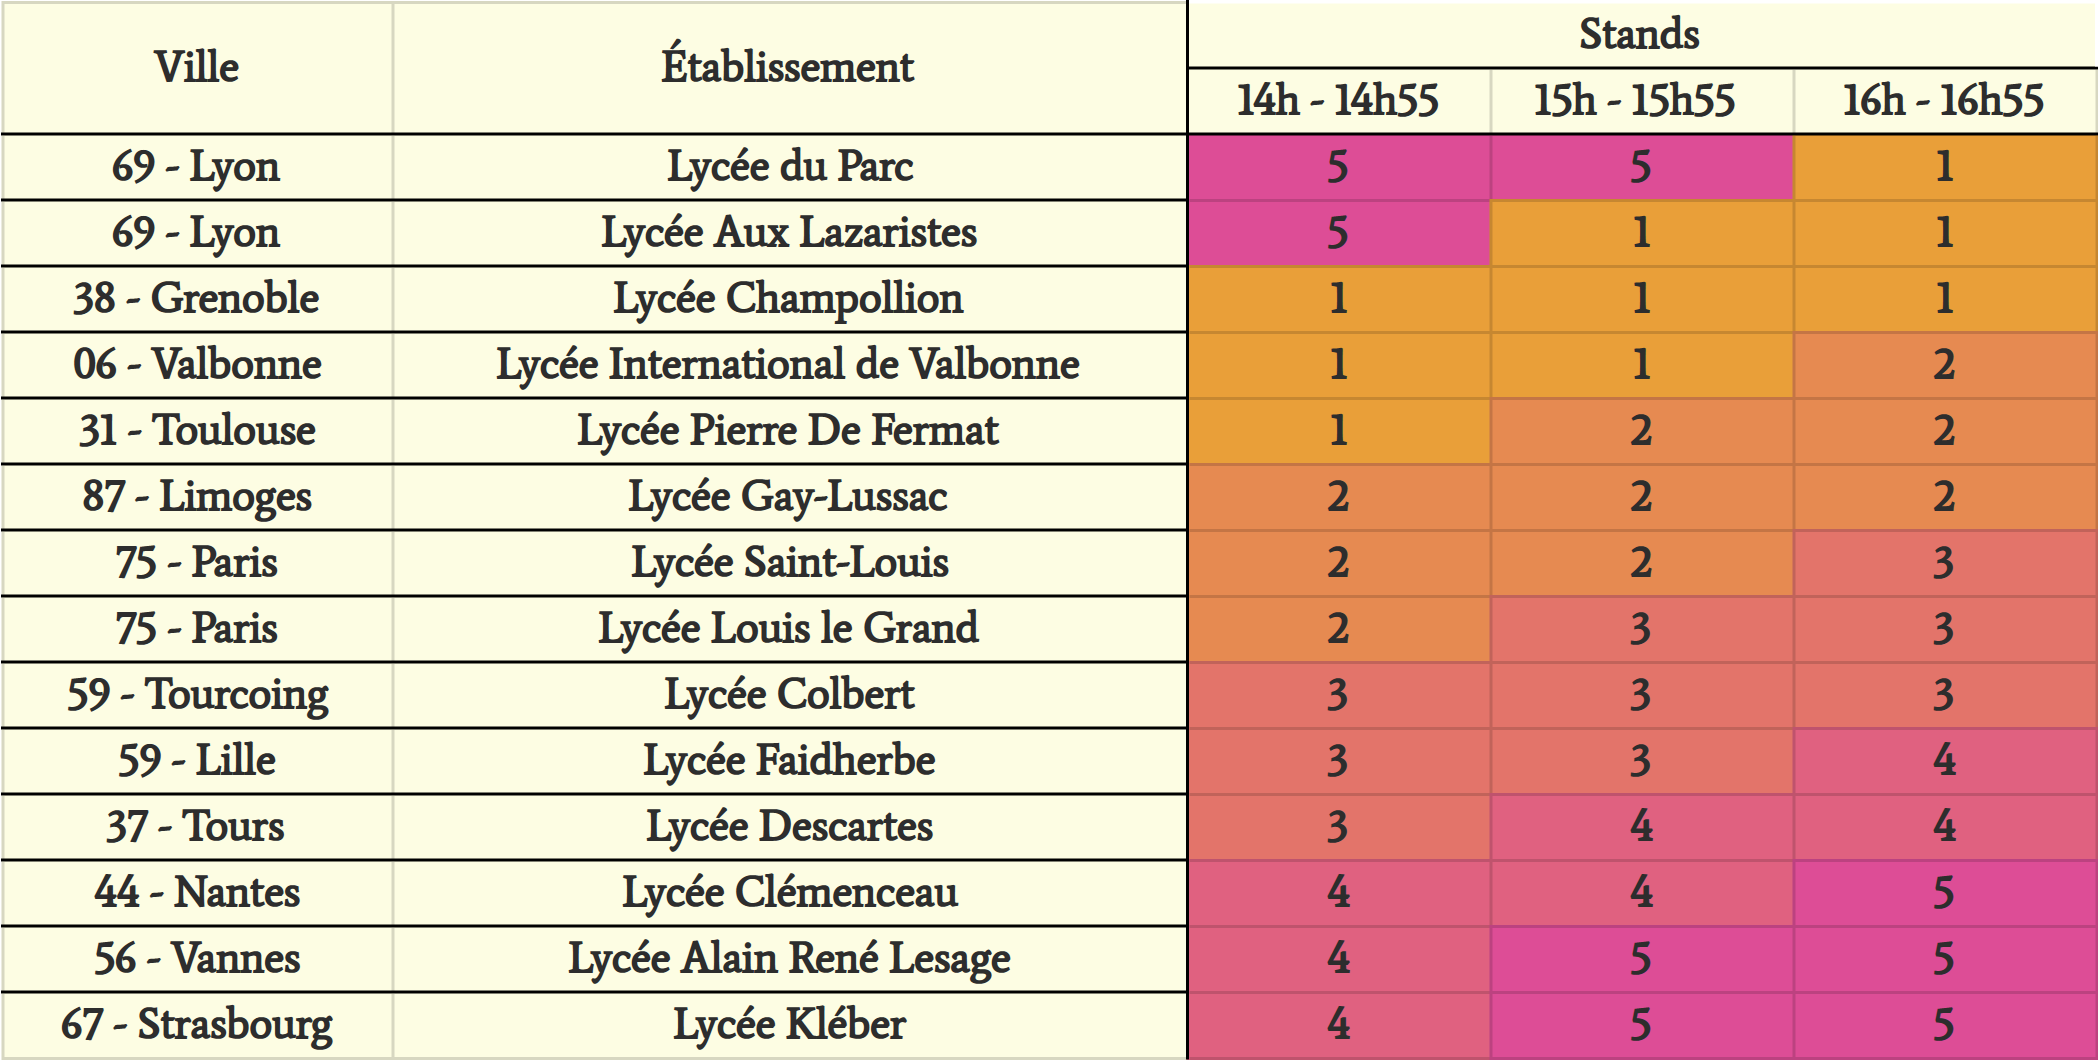
\includegraphics[width=0.9\textwidth]{ressource_diapo/Planing_2024.png}
        \caption{Planing du forum 2024 des MP2I-MPI}
    \end{figure}
\end{frame}

\section{statistiques}

\subsection{Resultats Parcoursup}

\begin{frame}
    \begin{figure}
        \centering
        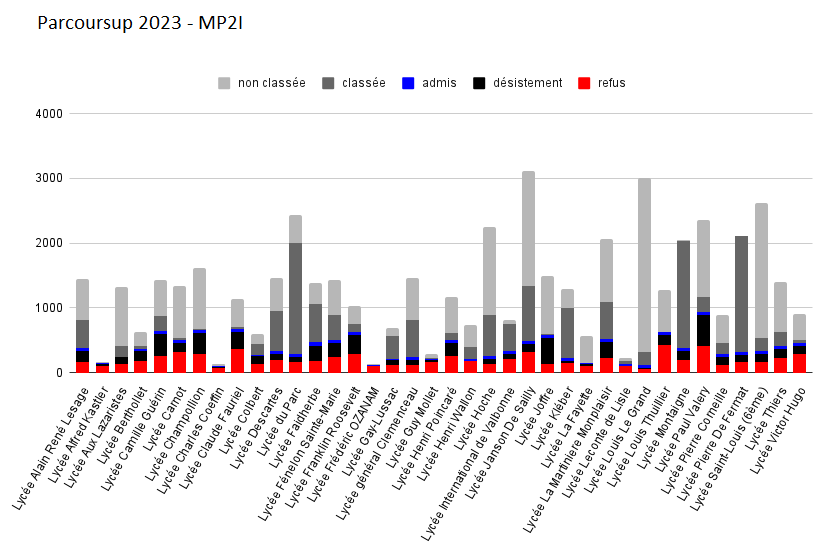
\includegraphics[width=0.9\textwidth]{ressource_diapo/Parcoursup_2023.png}
        \caption{Resultats Parcoursup}
    \end{figure}
\end{frame}

\subsection{Statistiques des mentions}

\begin{frame}
    \begin{figure}
        \centering
        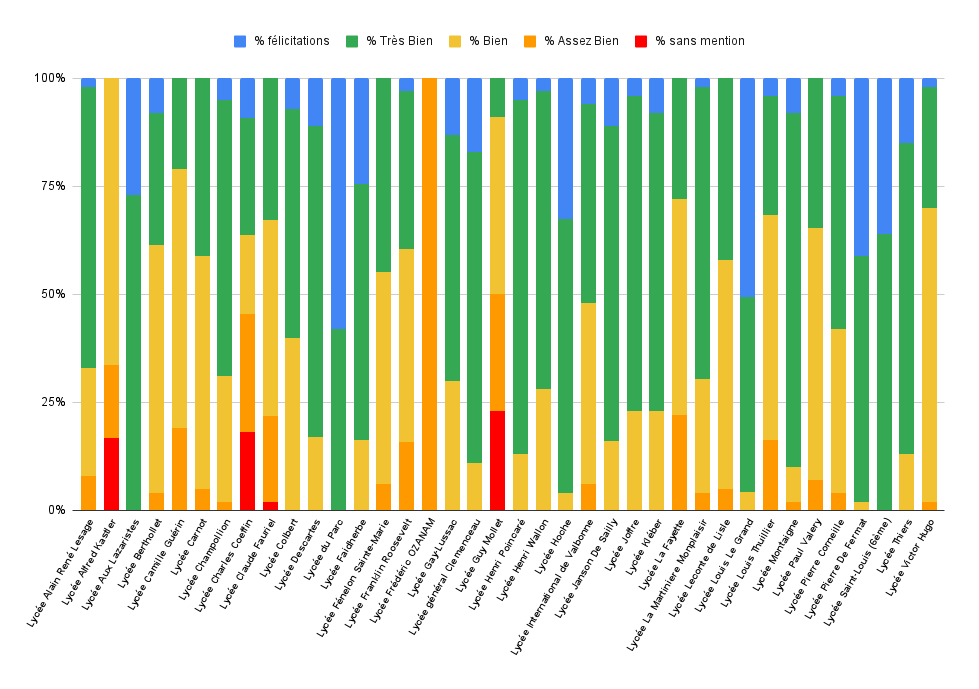
\includegraphics[width=0.9\textwidth]{ressource_diapo/mention 2023-2024.png}
        \caption{Statistiques des mentions}
    \end{figure}
\end{frame}

\subsection{Place en école d'ingénieur}

\begin{frame}
    \begin{itemize}
        \item \textbf{X} : 24 places
        \item \textbf{ENS} : ? places (Ulm : ?, Lyon : ?, Saclay : 8, Rennes : ?)
        \item \textbf{Centrales} : 118 places
        \item \textbf{Mines-Ponts} : 124 places
        \item \textbf{Mines-Télécom} : 141 places
        \item \textbf{CCINP} : 202 places (+22 autres écoles ratachées à CCINP)
        \item \textbf{E3A - polytech} : + de 160 places
    \end{itemize}
\end{frame}

\section{Différentes filières}

\subsection{Répartition horaire}

\begin{frame}
    \begin{figure}
        \centering
        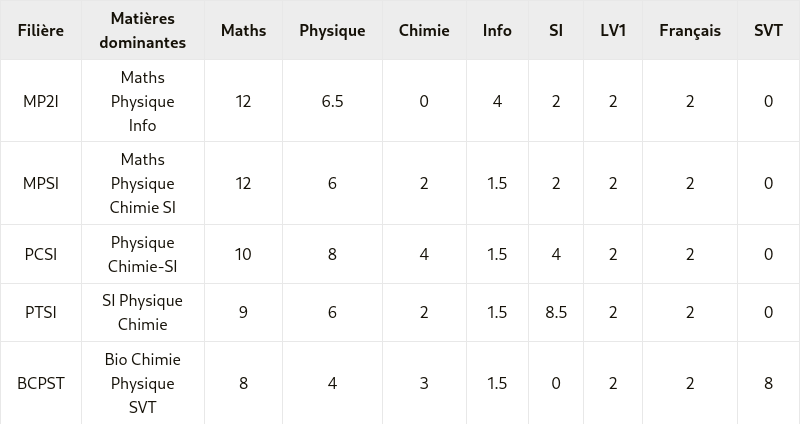
\includegraphics[width=\textwidth]{ressource_diapo/prepas.png}
        \caption{Répartition horaire}
    \end{figure}
\end{frame}

\subsection{Passage en deuxième année}

\begin{frame}
    \begin{figure}
        \centering
        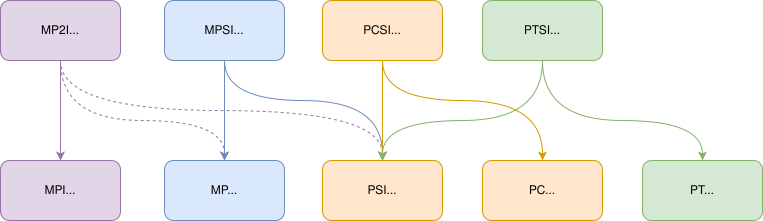
\includegraphics[width=\textwidth]{ressource_diapo/deuxieme_annee.png}
        \caption{Passage en deuxième année}
    \end{figure}
\end{frame}

\section{Vie en prépas}

\subsection{L'internat}

\begin{frame}
    \begin{figure}
        \centering
        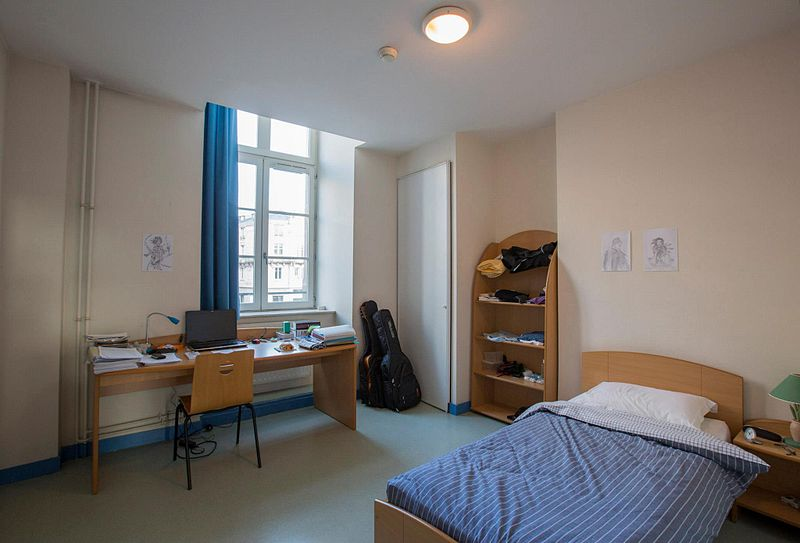
\includegraphics[width=0.9\textwidth]{ressource_diapo/Internat_Gay-Lussac_1.jpg}
        \caption{L'internat}
    \end{figure}
\end{frame}

\subsection{emploi du temps}

\begin{frame}
    \begin{figure}
        \centering
        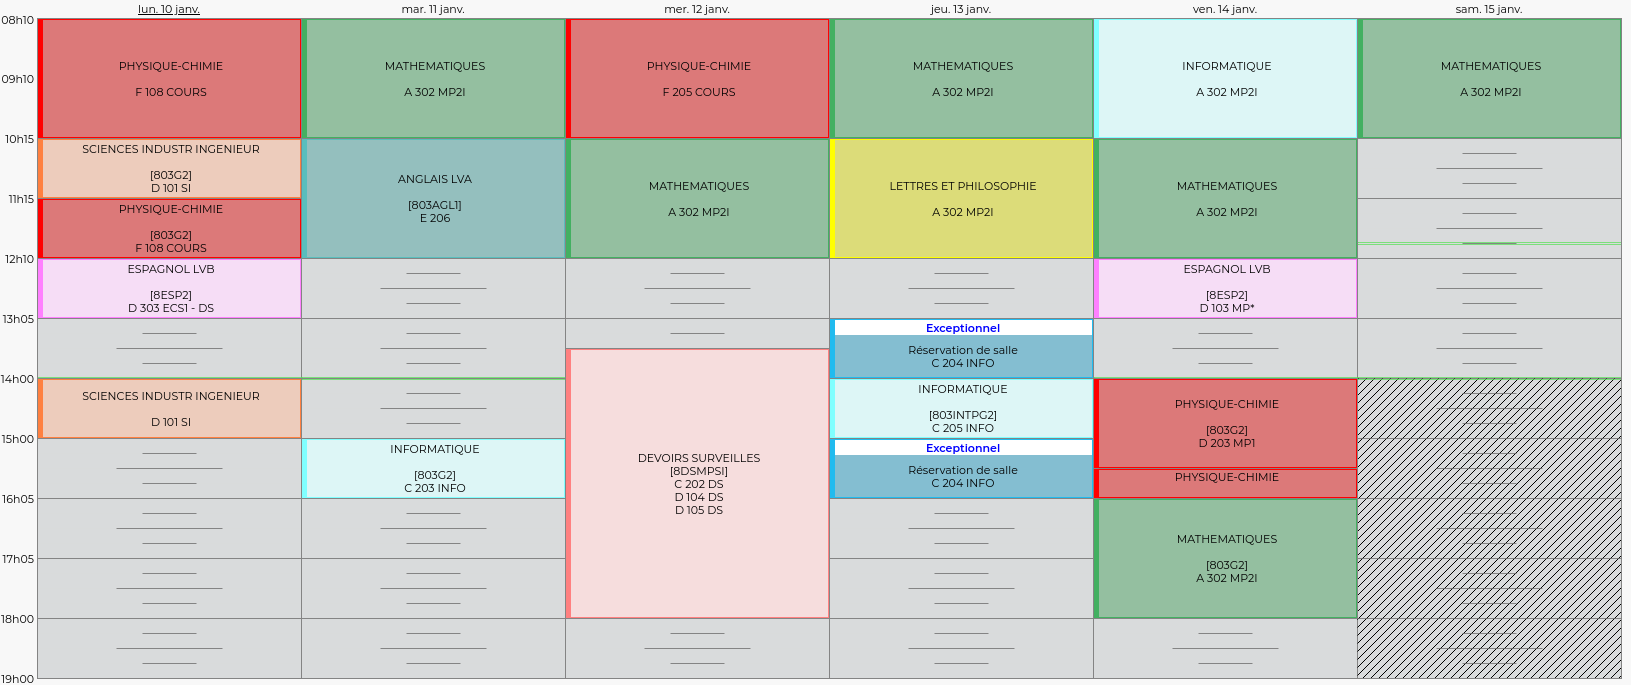
\includegraphics[width=0.9\textwidth]{ressource_diapo/emploi_du_temps.png}
        \caption{emploi du temps}
    \end{figure}
\end{frame}

\subsection{repartition aux concours}

\begin{frame}
    \begin{figure}[h]
        \begin{subfigure}{0.49\textwidth}
            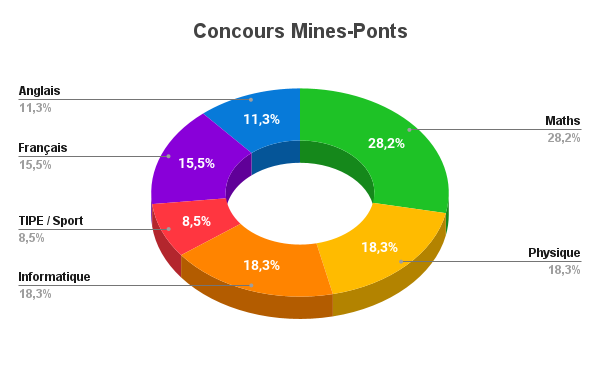
\includegraphics[width=0.95\linewidth]{ressource_diapo/Mines-Ponts.png}
        \end{subfigure}
        \begin{subfigure}{0.49\textwidth}
            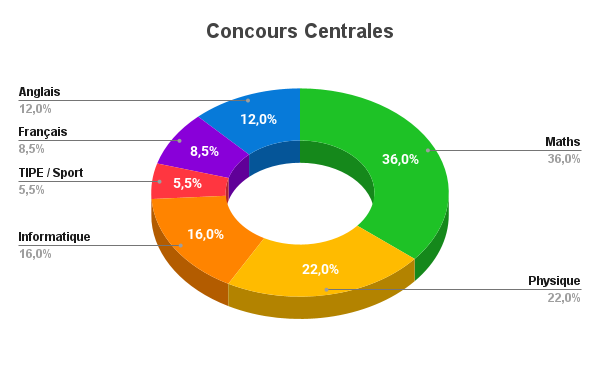
\includegraphics[width=0.95\linewidth]{ressource_diapo/Centrales.png}
        \end{subfigure}
        \begin{subfigure}{0.49\textwidth}
            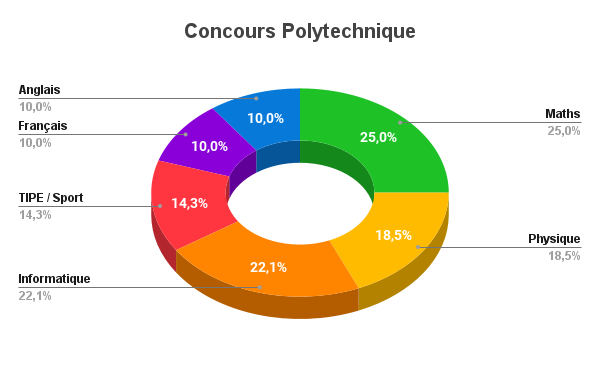
\includegraphics[width=0.95\linewidth]{ressource_diapo/X.png}
        \end{subfigure}
        \begin{subfigure}{0.49\textwidth}
            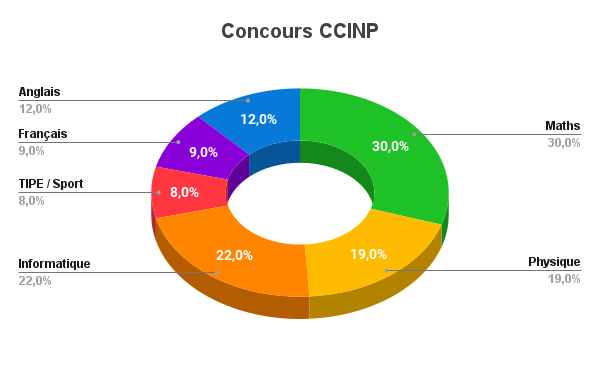
\includegraphics[width=0.95\linewidth]{ressource_diapo/CCINP.png}
        \end{subfigure}
    \end{figure}
\end{frame}

\section{Mathématiques}

\subsection{programme officiel S1}

\begin{frame}
    \textbf{Premier semestre}
    \begin{itemize}
        \item Raisonnements et vocabulaire ensembliste
        \item Compléments de calcul algébrique et de trigonométrie
        \item Nombres complexes
        \item Techniques fondamentales de calcul différentiel et intégral
        \item Nombres réels et suites géométriques
        \item Fonctions d'une variable réelle : continuité, dérivabilité, convexité
        \item Arithmétique dans l'ensemble des entiers relatifs
        \item Structures algébriques usuelles
        \item Calcul matriciel et systèmes linéaires
        \item Polynômes et fractions rationnelles
    \end{itemize}
\end{frame}

\subsection{programme officiel S2}

\begin{frame}
    \textbf{Deuxième semestre}
    \begin{itemize}
        \item Analyse asymptotique
        \item Espaces vectoriels et applications linéaires
        \item Matrices
        \item Groupe symétrique et déterminants
        \item Intégration
        \item Dénombrement
        \item Probabilités
        \item Espaces préhilbertiens réels
        \item Procédés sommatoires discrets
        \item Fonctions de deux variables
    \end{itemize}
\end{frame}

\section{Physique}

\subsection{programme officiel S1}

\begin{frame}
    \begin{enumerate}[label=\textbf{\arabic*.},leftmargin=*]
        \item \textbf{Ondes et signaux}
        \begin{enumerate}[label=1.\arabic*.]
            \item Formation des images
            \item Signaux et composants électriques
            \item Circuit linéaire du premier ordre et du deuxième ordre
            \item Propagation d'un signal
        \end{enumerate}
        \item \textbf{Mouvements et interactions}
        \begin{enumerate}[label=2.\arabic*.]
            \item Description et paramétrage du mouvement d’un point
            \item Lois de Newton
            \item Approche énergétique du mouvement d'un point matériel
            \item Mouvement de particules chargées dans des champs électrique et magnétostatique, uniformes et stationnaires 
        \end{enumerate}
        \item \textbf{L’énergie : conversions et transferts}
        \begin{enumerate}[label=3.\arabic*.]
            \item Descriptions microscopique et macroscopique d’un système : modèle du gaz parfait et de la phase condensée incompressible indilatable
            \item Bilan d’énergie pour un système thermodynamique
        \end{enumerate}    
    \end{enumerate}
\end{frame}

\subsection{programme officiel S2}

\begin{frame}
    \begin{enumerate}[label=\textbf{\arabic*.},leftmargin=*]
        \item \textbf{Ondes et signaux}
        \begin{enumerate}[label=1.\arabic*.]
            \item Régime sinusoïdal forcé
            \item Filtrage linéaire
            \item  Induction et forces de Laplace (champ magnétique, action d'un champ magnétique, lois de l'induction, Circuit fixe dans un champ magnétique qui dépend du temps et Circuit mobile dans un champ magnétique stationnaire)
            \item Introduction à la physique quantique
        \end{enumerate}
        \item \textbf{Mouvements et interactions}
        \begin{enumerate}[label=2.\arabic*.]
            \item Moment cinétique d’un point matériel
            \item Mouvements dans un champ de gravitation newtonien
            \item Mouvement d’un solide
        \end{enumerate}
        \item \textbf{L’énergie : conversions et transferts}
        \begin{enumerate}[label=3.\arabic*.]
            \item Deuxième principe. Bilans d'entropie
            \item Transitions de phases
            \item Machines thermiques 
        \end{enumerate}    
    \end{enumerate}
\end{frame}

\section{Informatique}

\subsection{programme officiel}

\begin{frame}
    \begin{enumerate}[label=\arabic*]
        \item Méthodes de programmation (S1) (S2) (S3-4)
        \item Récursivité et induction (S1) (S2)
        \item Structures de données (S1) (S2) (S3-4)
        \item Algorithmique (S2) (S3-4)
        \item Gestion des ressources de la machine (S1) (S3-4)
        \item Logique (S2) (S3-4)
        \item Bases de données (S2)
        \item Langages formels (S3-4)
        \item Décidabilité et classes de complexité (S3-4)
        \item Langage C et OCaml
    \end{enumerate}
\end{frame}

\subsection{Langage : Python}

\begin{frame}
    \begin{figure}
        \centering
        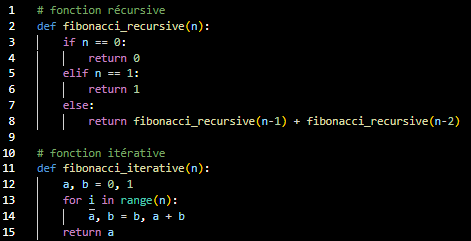
\includegraphics[width=0.9\linewidth]{ressource_diapo/fibo_python.PNG}
        \caption{Deux versions de la fonction fibonacci en python}
    \end{figure}
    Le Python n'est pas au programme d'informatique, mais il peut apparaître dans des épreuves de mathématiques ou de physique lors des concours.
\end{frame}

\subsection{Langage : OcamL}

\begin{frame}
    \begin{figure}
        \centering
        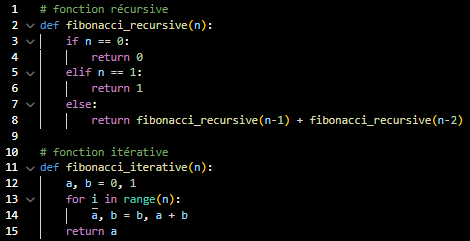
\includegraphics[width=0.9\linewidth]{ressource_diapo/fibo_ocaml.PNG}
        \caption{Deux versions de la fonction fibonacci en ocaml}
    \end{figure}
\end{frame}

\subsection{Langage : C}

\begin{frame}
    \begin{figure}
        \centering
        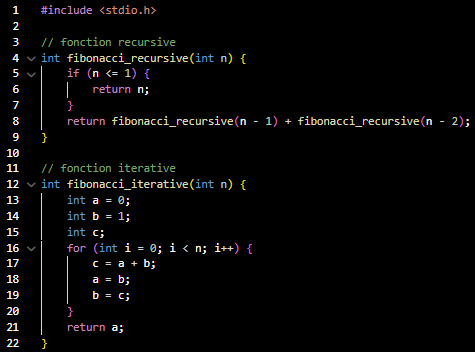
\includegraphics[width=0.9\linewidth]{ressource_diapo/fibo_c.PNG}
        \caption{Deux versions de la fonction fibonacci en C}
    \end{figure}
\end{frame}

\section{FAQ}

\subsection{avant la prépa}

\begin{frame}
    \textbf{Avant la prépa :}
    \begin{itemize}
        \item \textbf{Sélection} : \textit{Mention au bac ? Niveau/classement en terminale ? Lettre de motivation ?}
        \item \textbf{Choix des spécialité} : \textit{Quelle spécialité choisir pour une prépa MP2I-MPI? NSI, SI, Maths, Physique, Informatique? Maths expertes? pratique de l'informatique avant la prépa?}
        \item \textbf{Préparer la prépa} : \textit{Comment se préparer à la prépa? Réviser le programme de terminale? S'avancer sur le programme de prépa? Profiter de ses vacances? S'entrainer à coder? Lire les livres de français?}
    \end{itemize}
\end{frame}

\subsection{pendant la prépa}

\begin{frame}
    \textbf{En prépa :}
    \begin{itemize}
        \item \textbf{Rythme} : \textit{Emploi du temps ? Vitesses des cours ? Rythme le week-end ? En vacances ? Travail en dehors des cours ? Activité sportive ?}
        \item \textbf{Matières} : \textit{LV2 ? TIPE ? Khôlles ? Philo ? Anglais ? Maths ? Physique ? Chimie ? Info ?}
        \item \textbf{L'ambiance} : \textit{Les profs sont méchants ? Entraide ? Amis ? Concurrence dans la classe ?}
        \item \textbf{Se loger} : \textit{Internat ? Appartement ?  Collocation ? Durée de trajet ? Rentrer le week-end ?}
        \item \textbf{Internat} : \textit{Ouvert le week-end/vacances ? Inter-externé/externe/interne ? Ambiance et travail ?}
        \item \textbf{Débouchés} : \textit{Concours ? Réorientation ? 5/2 ? Quels métiers ?}
    \end{itemize}
\end{frame}

\subsection{en MP2I}

\begin{frame}
    \textbf{En MP2I :}
    \begin{itemize}
        \item \textbf{Info théorique} : \textit{TD sur papier ? Algo sur papier ? Quel est le programme ? Que faites-vous ?}
        \item \textbf{Info pratique} : \textit{OCaml ? C ? Programmation fonctionnelle/impérative ?}
        \item \textbf{Math} : \textit{Quelle est le programme en maths comparé aux MPSI ?}
        \item \textbf{Physique} : \textit{Programme ? Chimie ? Python ? }
        \item \textbf{Choix de spé} : \textit{MPI/MP/PSI ? Université ? Classe étoilée ?}
    \end{itemize}
\end{frame}

\section{Annexe}

\begin{frame}
    \begin{figure}
        \centering
        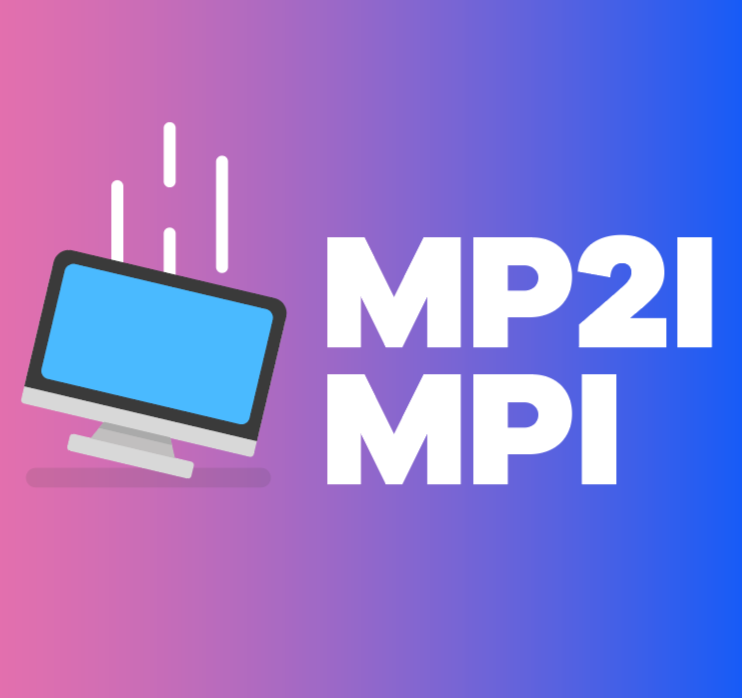
\includegraphics[width=0.35\textwidth]{ressource_diapo/logo_discord.png}
    \end{figure}
    \textbf{Notre discord :} \textit{https://discord.gg/Mu439mBdsv}\\
    \textbf{Notre site :} \textit{https://prepas-mp2i.fr}
\end{frame}

\end{document}
